\section{Comparative Analysis of Representative Systems}\label{sec:taxonomy}
The literature on world modeling in dynamic environments spans a wide range of representational choices, inference strategies and application targets.
While individual systems are often described in isolation, a comparative perspective is necessary to understand how these design decisions relate to one another and how different combinations of graphical models, dynamic handling, and uncertainty profiles emerge in practice. 
This section provides a structured comparison of the surveyed \emph{systems} themselves, classifying graph-based dynamic world models for robotics along a set of common axes.
Rather than ranking methods by performance, the comparison aims to map the design space, highlighting recurring architectural patterns and characteristic trade-offs across factor-graph-based, scene-graph-based and hybrid representations.

\subsection{Axes of Comparison}\label{sec:taxonomy_axes}
The analysis organizes existing approaches along several dimensions that recur throughout the surveyed literature:
\begin{itemize}
    \item \textbf{Graph Stack}: the primary representational backbone employed by the system, distinguishing between factor graphs (FG), scene graph (SG), and hybrid architectures that explicitly maintain both representations with cross-representation correspondence, as defined in Section \ref{sec:background_hybrid};
    \item \textbf{Dynamics Type}: the class of environmental change modeled, using the same three-tier Temporal Horizon distinction introduced in Section \ref{sec:taxonomy_dynamics} (short-term dynamics, semi-static changes, and long-term structural evolution);
    \item \textbf{Represented Scene}: the operational context, such as indoor, outdoor, or any environment;
    \item \textbf{Data Association Strategy}: the mechanism used to link observations over time, ranging from deterministic matching to probabilistic multi-hypothesis methods or learned similarity models;
    \item \textbf{Inference Policy}: the underlying inference method, including batch maximum a posteriori (MAP) optimization, incremental smoothing, filtering-based approaches, or variational inference;
    \item \textbf{Uncertainty Profile}:  which uncertainty classes are represented (\textit{geometric state, \textit{semantics}, \textit{data association}, \textit{existence}, and \textit{relations}), and whether their treatment is explicitly probabilistic, heuristic or deterministic};
    \item \textbf{Sensor}: the employed sensing inputs used to build the world model;
    \item \textbf{System Properties}: 
    \begin{itemize}
        \item \textbf{RT} denotes reported real-time operation under the hardware, sensing configuration, scene complexity, and experimental conditions of the original work. It is therefore not a normalized cross-method performance comparison. \checkmark~ indicates that end-to-end online operation was experimentally demonstrated at the operating rate reported by the authors; $\sim$ indicates partial/module-level real-time operation or architectural support without end-to-end demonstration; \xmark~ indicates that real-time was not demonstrated or reported.
        \item \textbf{OV}: \checkmark~ requires experimental operation beyond a fixed predefined semantic vocabulary; $\sim$ denotes use of open-vocabulary components without end-to-end evaluation; \xmark~ denotes no reported demonstration.
        \item \textbf{MR}: \checkmark~ requires an experimental demonstration in which multiple robots collaboratively construct, update, or use a shared representation; $\sim$ denotes architectural or component-level multi-robot support without end-to-end demonstration; \xmark~ denotes no reported demonstration.
    \end{itemize}
    \item \textbf{Downstream Usage}: the primary tasks specifically enabled or targeted by the representation, such as robust SLAM, navigation, manipulation, interaction understanding, or prediction. This axis identifies the intended use of the representation and should not by itself be considered as evidence of improved task-level performance; such evidence requires an explicit task-level evaluation as defined in Section \ref{sec:evaluation_metrics}. 
\end{itemize}
These axes stem from the three research questions posed in Section \ref{sec:introduction}: Graph Stack, Dynamics Type, and Represented Scene characterize \emph{what is represented} (RQ1); Data Association Strategy, Inference Policy, Uncertainty Profile, and Sensor  characterize \emph{how the representation is constructed and maintained} (RQ2); and System Properties, and Downstream Usage characterize \emph{how the representation is exploited} (RQ3). 
Together, these axes provide a unified lens through which heterogeneous systems can be compared across all three questions simultaneously, without assuming a notion of optimality.

\subsection{Comparison of Existing Approaches}\label{sec:taxonomy_taxonomy}
Table \ref{tab:taxonomy_overview} summarizes representative works in the literature according to the comparison dimensions defined above.
The listed systems are grouped by their underlying graph stack, enabling a direct comparison between factor-graph-based methods, scene-graph-centric approaches, and hybrid representations that integrate probabilistic estimation with semantic abstraction.
Because the surveyed systems are evaluated using different sensors, datasets, tasks, and metrics, this comparison supports an architectural analysis rather than a performance ranking. 
The comparison axes should not be interpreted as implying a common objective across all representational paradigms.
Dimensions such as sensing, dynamics coverage, data-association strategy, system properties and downstream usage can be compared descriptively across architectures, whereas inference policy and uncertainty profile characterize paradigm-specific mechanisms rather than values on a common performance scale. 
For example, learned semantic confidence scores, language-model outputs, and covariance-based probabilistic estimates represent fundamentally different quantities and should not be treated as equivalent uncertainty measures.
Accordingly, the reported system-property indicators summarize the level of evidence provided by the original works under their evaluated configurations, rather than intrinsic system capabilities, and differences in reported downstream performance cannot generally be attributed to the representation choice alone.
Moreover, the surveyed literature does not provide a standardized metric or controlled benchmark that isolates the effect of the representation architecture itself.
Existing metrics quantify individual aspects, such as geometric accuracy or downstream task success, but do not define a common measure of superiority across FG, SG, and hybrid FG-SG architectures.

\begin{table*}[htbp]
\caption{Comparative analysis of representative
probabilistic graph-based \emph{systems} for robotics in dynamic
environments.}
  \label{tab:taxonomy_overview}
  \centering

  \adjustbox{max width=\textwidth, max totalheight=0.85\textheight}{%
  \scriptsize
  \setlength{\tabcolsep}{2pt}
  \renewcommand{\arraystretch}{0.2}
  \setlength{\extrarowheight}{-2pt}
  \setlength{\aboverulesep}{0.2ex}

    \begin{tabularx}{\textwidth}{@{}
      >{\raggedright\arraybackslash}l  % Work
      >{\centering\arraybackslash}p{1.0cm}   % Graph stack 
      >{\raggedright\arraybackslash}X        % Nodes
      >{\raggedright\arraybackslash}X        % Edges
      >{\raggedright\arraybackslash}X        % Dynamics type
      >{\raggedright\arraybackslash}X        % Represented scene
      >{\raggedright\arraybackslash}X        % Association
      >{\raggedright\arraybackslash}X        % Inference
      >{\raggedright\arraybackslash}X        % Uncertainty
      >{\raggedright\arraybackslash}X        % Sensors
      c c c                                  % RT OV MR
      >{\raggedright\arraybackslash}X@{}     % Downstream use
    }
    \toprule
    & \multicolumn{5}{c}{\textbf{Representation}} &
    \multicolumn{4}{c}{\textbf{Construction \& Maintenance}} &
    \multicolumn{4}{c}{\textbf{Exploitation}} \\
    \cmidrule(lr){2-6} \cmidrule(lr){7-10} \cmidrule(lr){11-14}
    \textbf{Work} & \textbf{Graph stack} & \textbf{Nodes} & \textbf{Edges} & \textbf{Dynamics type} &
    \textbf{Represented scene} &
    \textbf{Association} & \textbf{Inference} & \textbf{Uncertainty Profile} & \textbf{Sensors} &
    \textbf{RT} & \textbf{OV} & \textbf{MR} & \textbf{Downstream use} \\
    \midrule

    % ── FACTOR GRAPH ONLY ──────────────────────────────────────────────────────
    \multicolumn{14}{@{}c}{\textit{Factor graph (FG) only}} \\
    \midrule

    \makecell[l]{DynaSLAM II\\Bescos et al.\\ (2021)\cite{bescos_dynaslam_2021}} &
    \makecell[c]{FG} &
    \makecell[l]{Camera pose,\\object pose, \\velocity,\\points} &
    \makecell[l]{reprojection \\error,\\motion error} &
    \makecell[l]{short-term \cmark\\semi-static \xmark\\long-term \xmark} &
    Outdoor &
    \makecell[l]{deterministic\\(ORB + IoU)} &
    \makecell[l]{batch\\MAP} &
    \makecell[l]{G:P, S:D,\\ A:D, E:D,\\ R:--} &
    \makecell[l]{Stereo or\\RGB-D} &
    \cmark & \xmark & \xmark &
    \makecell[l]{Collision \\avoidance\\+ SLAMMOT} \\
    \midrule

    \makecell[l]{Brink\\(2016)\cite{brink_using_2016}} &
    \makecell[c]{FG} &
    \makecell[l]{Image features,\\velocity} &
    \makecell[l]{same-object\\probabilistic\\ dependency} &
    \makecell[l]{short-term \cmark\\semi-static  \xmark\\long-term \xmark} &
    Any &
    \makecell[l]{deterministic\\(Delaunay\\ triangulation)} &
    \makecell[l]{incremental\\loopy BP} &
    \makecell[l]{G:P, S:--,\\ A:D, E:--,\\ R:--} &
    \makecell[l]{Stereo} &
    \xmark & \xmark & \xmark &
    \makecell[l]{Dynamic\\ object\\detection} \\
    \midrule

    \makecell[l]{DynoSAM\\Morris et al.\\(2025)\cite{morris_dynosam_2025}} &
    \makecell[c]{FG} &
    \makecell[l]{Camera poses,\\object \\motions/poses,\\map points} &
    \makecell[l]{point meas.,\\ odometry,\\object motion,\\ obj. smoothing,\\prior factors} &
    \makecell[l]{short-term \cmark\\semi-static \xmark\\long-term \xmark} &
    Any &
    \makecell[l]{optical flow\\+ instance seg.} &
    \makecell[l]{\\ full-batch\\smoothing} &
    \makecell[l]{G:P, S:D,\\ A:D, E:D,\\ R:--} &
    \makecell[l]{RGB-D} &
    \xmark & \xmark & \xmark &
    \makecell[l]{4D dynamic\\reconstruction} \\
    \midrule

    \makecell[l]{Gou et al.\\(2024)\cite{gou_visual_2024}} &
    \makecell[c]{FG} &
    \makecell[l]{Camera poses,\\landmarks,\\ objects} &
    \makecell[l]{static reproj.,\\ camera meas.,\\dynamic reproj.,\\ object motion} &
    \makecell[l]{short-term \cmark\\semi-static \xmark\\long-term \xmark} &
    Any &
    \makecell[l]{Hungarian\\algorithm} &
    \makecell[l]{local/global\\BA} &
    \makecell[l]{G:P, S:D,\\ A:D, E:D,\\ R:--} &
    \makecell[l]{RGB-D} &
    \xmark & \xmark & \xmark &
    \makecell[l]{Industrial\\inspection} \\
    \midrule

    \makecell[l]{Gomez et al.\\(2020)\cite{gomez_object-based_2020}} &
    \makecell[c]{FG} &
    \makecell[l]{Poses,\\ objects\\(cuboid\\ centroids)} &
    \makecell[l]{ pose-pose,\\  pose-object\\  obs. links } &
    \makecell[l]{short-term \xmark\\semi-static \cmark\\long-term \xmark} &
     Indoor &
    \makecell[l]{area of\\influence} &
    \makecell[l]{multi-session\\  probabilistic \\ map update} &
    \makecell[l]{G:D, S:D,\\ A:D, E:P,\\ R:--} &
    \makecell[l]{RGB-D} &
    \xmark & \xmark & \xmark &
    \makecell[l]{Autonomous\\ indoor\\service robots} \\
    \midrule

    % \makecell[l]{Zaech et al.\\(2022)\cite{zaech_learnable_2022}} &
    % \makecell[c]{FG} &
    % \makecell[l]{Object\\ observations,\\object tracks} &
    % \makecell[l]{data\\association} &
    % \makecell[l]{short-term \cmark\\semi-static \xmark\\long-term \xmark} &
    % Any &
    % \makecell[l]{learned\\ matching\\(NMP)} &
    % \makecell[l]{filtering\\(Kalman)} &
    % \makecell[l]{G:P, S:D,\\ A:H, E:H,\\ R:--} &
    % \makecell[l]{LiDAR} &
    % \cmark & \xmark & \xmark &
    % \makecell[l]{3D multi-object\\tracking} \\
    % \midrule

    \makecell[l]{BodySLAM\\Henning et al.\\(2022)\cite{henning_bodyslam_2022}} &
    \makecell[c]{FG} &
    \makecell[l]{Camera poses,\\human centre\\poses, SMPL\\body params} &
    \makecell[l]{reprojection\\error, human\\motion model\\(temporal)} &
    \makecell[l]{short-term \cmark\\semi-static \xmark\\long-term \xmark} &
    Any &
    \makecell[l]{OpenPose\\keypoints} &
    \makecell[l]{batch\\MAP} &
    \makecell[l]{G:H, S:D,\\ A:--, E:--,\\ R:--} &
    \makecell[l]{Monocular} &
    \xmark & \xmark & \xmark &
    \makecell[l]{Human pose\\+ camera\\trajectory\\estimation} \\
    \midrule

    \makecell[l]{BodySLAM++\\Henning et al.\\(2023)\cite{henning_bodyslam_2023}} &
    \makecell[c]{FG} &
    \makecell[l]{Camera poses,\\IMU states,\\human pose\\+shape(SMPL)} &
    \makecell[l]{repr. error,\\ IMU factors,\\human motion\\constraints} &
    \makecell[l]{short-term \cmark\\semi-static \xmark\\long-term \xmark} &
    Indoor &
    \makecell[l]{learned\\(HMR)} &
    \makecell[l]{incremental\\smoothing\\(OKVIS2)} &
    \makecell[l]{G:P/H, S:D,\\ A:D, E:D,\\ R:--} &
    \makecell[l]{Monocular\\+ IMU} &
    \cmark & \xmark & \xmark &
    \makecell[l]{Real-time\\human +\\camera state\\estimation} \\
    \midrule

    \makecell[l]{AirDOS\\Qiu et al.\\(2022)\cite{qiu2022airdos}} &
    \makecell[c]{FG} &
    \makecell[l]{Camera poses,\\object motion,\\rigid part\\structure\\(3D points)} &
    \makecell[l]{rigidity and\\motion\\constraints,\\reprojection\\error} &
    \makecell[l]{short-term \cmark\\semi-static \xmark\\long-term \xmark} &
    Outdoor &
    \makecell[l]{ORB features\\+ instance\\segmentation} &
    \makecell[l]{batch\\MAP} &
    \makecell[l]{G:P, S:D,\\ A:D, E:D,\\ R:--} &
    \makecell[l]{Stereo} &
    \xmark & \xmark & \xmark &
    \makecell[l]{4D spatio-\\temporal maps,\\crowded\\urban SLAM} \\
    \midrule

    % ── HYBRID ─────────────────────────────────────────────────────────────────
    \multicolumn{14}{@{}c}{\textit{Hybrid (FG + SG)}} \\
    \midrule

    \makecell[l]{DynEMo-SLAM\\Giberna et al.\\(2025)\cite{giberna_dynemo-slam_2025}} &
    \makecell[c]{Hybrid} &
    \makecell[l]{Keyframes,\\ entity obs.,\\planes, floor} &
    \makecell[l]{KF-entity,\\intra-entity,\\floor-entity} &
    \makecell[l]{short-term \cmark\\semi-static \cmark\\long-term \xmark} &
    Indoor &
    \makecell[l]{deterministic\\(AprilTags)} &
    \makecell[l]{global nonlinear\\ graph opt.} &
    \makecell[l]{G:P, S:D,\\ A:D, E:--,\\ R:D} &
    \makecell[l]{LiDAR +\\camera} &
    \cmark & \xmark & \xmark &
    \makecell[l]{Metric-semantic\\reconstruction in\\crowded envs.} \\
    \midrule

    \makecell[l]{Kimera\\Rosinol et al.\\(2021)\cite{rosinol_kimera_2021}} &
    \makecell[c]{Hybrid} &
    \makecell[l]{Free space,\\agents/objects,\\rooms,\\ building} &
    \makecell[l]{Semantic\\ relations} &
    \makecell[l]{short-term \cmark\\semi-static \xmark\\long-term \xmark} &
    Indoor &
    \makecell[l]{TEASER++\\+ seg.} &
    \makecell[l]{iSAM2 +\\batch parsing} &
    \makecell[l]{G:P, S:P,\\ A:D, E:--,\\ R:D} &
    \makecell[l]{Vis.-inertial\\+ RGB-D} &
    $\sim$ & \xmark & \xmark &
    \makecell[l]{Hierarchical\\ metric-semantic\\reconstruction \\+ planning} \\
    \midrule

    \makecell[l]{Khronos\\Schmid et al.\\(2024)\cite{schmid_khronos_2024}} &
    \makecell[c]{Hybrid} &
    \makecell[l]{Poses, objects,\\object\\ fragments} &
    \makecell[l]{associations,\\odometry} &
    \makecell[l]{short-term \cmark\\semi-static \cmark\\long-term \xmark} &
    Indoor &
    \makecell[l]{volumetric IoU\\(multi-hyp.)} &
    \makecell[l]{async global\\optimization} &
    \makecell[l]{G:P, S:D,\\ A:P, E:H,\\ R:--} &
    \makecell[l]{RGB-D} &
    \cmark & \cmark & \xmark &
    \makecell[l]{ spatio-temporal\\mapping +\\ change detect.} \\
    \midrule

    % ── SCENE GRAPH ONLY ───────────────────────────────────────────────────────
    \multicolumn{14}{@{}c}{\textit{Scene graph (SG) only}} \\
    \midrule

    \makecell[l]{Lost \& Found\\Behrens et al.\\ (2025)\cite{behrens_lost_2025}} &
    \makecell[c]{SG} &
    \makecell[l]{Objects,\\ object parts,\\points} &
    \makecell[l]{Semantic\\ spatial\\ relations} &
    \makecell[l]{short-term \cmark\\semi-static \cmark\\long-term \xmark} &
    Indoor &
    \makecell[l]{image-based\\detection} &
    \makecell[l]{visual point\\tracking} &
    \makecell[l]{G:D, S:D,\\ A:H, E:D\\ R:D} &
    \makecell[l]{RGB-D} &
    $\sim$ & \xmark & \xmark &
    \makecell[l]{Object\\ tracking +\\manipulation} \\
    \midrule

    \makecell[l]{DovSG\\Yan et al.\\(2025)\cite{yan_dynamic_2025}} &
    \makecell[c]{SG} &
    \makecell[l]{Objects\\ (labels,\\color,\\ material)} &
    \makecell[l]{Semantic\\ spatial\\ relations} &
    \makecell[l]{short-term  \xmark\\semi-static \cmark \\long-term \xmark} &
    Indoor &
    \makecell[l]{similarity-based\\(CLIP features)} &
    \makecell[l]{online logic\\updates} &
    \makecell[l]{G:D, S:H,\\ A:H, E:D\\ R:D} &
    \makecell[l]{RGB-D} &
    $\sim$ & \cmark & \xmark &
    \makecell[l]{Mobile\\ manipulation\\+ task\\ planning} \\
    \midrule

    \makecell[l]{CURB-SG\\Greve et al.\\(2024)\cite{greve_collaborative_2024}} &
    \makecell[c]{ Hybrid} &
    \makecell[l]{Environment,\\roads and\\ intersections,\\landmarks} &
    \makecell[l]{spatial\\ relations} &
    \makecell[l]{short-term \cmark\\semi-static \xmark\\long-term \xmark} &
    Outdoor &
    \makecell[l]{scan match.\\+ local search} &
    \makecell[l]{pose graph\\opt. (PGO)} &
    \makecell[l]{G:P, S:D,\\ A:H, E:--\\ R:D} &
    \makecell[l]{LiDAR} &
    \xmark & \xmark & \cmark &
    \makecell[l]{Automated\\driving} \\
    \midrule

    \makecell[l]{Aion\\Catalano et al.\\(2025)\cite{catalano_aion_2025}} &
    \makecell[c]{SG} &
    \makecell[l]{Entity obs.,\\navigational\\ flows, semantic\\ abstraction} &
    \makecell[l]{spatial/semantic\\ rels., planning\\ connectivity,\\traversal costs} &
    \makecell[l]{short-term \cmark\\semi-static \xmark\\long-term \xmark} &
    Indoor &
    \makecell[l]{pos.-invariant\\indexing} &
    \makecell[l]{FreMEn\\(frequency)} &
    \makecell[l]{G:P, S:D,\\ A:D, E:--\\ R:D} &
    \makecell[l]{RGB-D /\\Stereo} &
    $\sim$ & \xmark & \xmark &
    \makecell[l]{Forecasting\\ human\\activity for\\ navigation} \\
    \midrule

    \makecell[l]{Functional SG\\Zhang et al.\\(2025)\cite{zhang_open-vocabulary_2025}} &
    \makecell[c]{SG} &
    \makecell[l]{Objects and\\interactive\\ elements} &
    \makecell[l]{functional\\relationships} &
    \makecell[l]{short-term \xmark\\semi-static \cmark\\long-term \xmark} &
    Indoor &
    \makecell[l]{learned\\matching} &
    \makecell[l]{sequential\\LLM reasoning} &
    \makecell[l]{G:D, S:H,\\ A:H, E:--\\ R:H} &
    \makecell[l]{RGB-D} &
    \xmark & \xmark & \xmark &
    \makecell[l]{3D VQA\\+ manipulation} \\
    \midrule

    \makecell[l]{Saucedo et al.\\(2025)\cite{saucedo_estimating_2025}} &
    \makecell[c]{SG (BSG)} &
    \makecell[l]{Building,\\ rooms,\\objects} &
    \makecell[l]{Semantic and\\ geometric\\ spatial rel.} &
    \makecell[l]{short-term \xmark\\semi-static \cmark\\long-term \xmark} &
    Indoor &
    \makecell[l]{learned\\matching} &
    \makecell[l]{variational\\(GCN pred.)} &
    \makecell[l]{G:P, S:D,\\ A:--, E:--\\ R:D} &
    \makecell[l]{RGB-D} &
    \xmark & \cmark & \xmark &
    \makecell[l]{Unvisited\\ scene\\completion}\\
    \bottomrule
    \end{tabularx}
    } % end adjustbox
  \vspace{2pt}
  {\scriptsize
  \begin{tabularx}{\textwidth}{@{}l >{\raggedright\arraybackslash}X@{}}
    \textbf{Legend:} &
    \textbf{Graph stack}: FG (factor graph), SG (scene graph), Hybrid (FG-backed SG / SG-constrained FG).
    \textbf{Dynamics type}: (i) short-term, (ii) semi-static,    (iii)  long-term structural change.
    \textbf{Represented Scene}: Indoor, Outdoor, Any.
    \textbf{Association}: data association (deterministic, MHT, JPDA, learned matching).
    \textbf{Inference}: batch MAP, incremental smoothing, filtering, variational, particle/mixture.
    \textbf{Uncertainty Profile}: G = geometric-state uncertainty; S = semantic uncertainty; A = data-association uncertainty; E = existence uncertainty; R = relational uncertainty. P = explicit probabilistic treatment; H = heuristic or uncalibrated confidence; D = deterministic treatment; -- = uncertainty class not explicitly represented or reported.
    \textbf{RT/OV/MR}: real-time / open-vocabulary / multi-robot; \cmark = experimentally demonstrated, $\sim$ = partially demonstrated or supported/claimed but not demonstrated end-to-end, \xmark = not demonstrated/reported. RT is configuration-specific, OV requires operation beyond a fixed vocabulary, MR requires collaborative multi-robot operation. \\
  \end{tabularx}
  }
\end{table*}

The table illustrates the variety of design choices explored, from tightly-coupled SLAMMOT systems that extend classical factor graphs with dynamic entity modeling, to scene-graph-based frameworks emphasizing semantic structure and interaction, finally to hybrid systems that combine geometric consistency with relational reasoning.

\subsection{Cross-Comparison}\label{sec:taxonomy_crosscomparison}
Across the surveyed works, four recurring architectural patterns emerge, as shown in Figure \ref{fig:architectural_patterns}, distinguished primarily by the representational stack  and, for hybrid systems, by the coupling between the FG and SG components. 
We classify each representative implementation according to the information flow and optimization structure reported for that system.
For the higher-level comparison in this section, the feed-forward layered and parallel architectures introduced in Section \ref{sec:background_hybrid} are grouped under the broader loosely coupled hybrid class, since in both cases the FG and SG remain outside a single joint optimization.
The tightly coupled class instead requires scene-graph-level entities or constraints to participate directly in the estimation graph.
% Two patterns rely on a single representational backbone, factor graphs alone or scene graphs alone, while two combine both, differing in whether information flows in one direction or both.

\begin{figure}
    \centering
    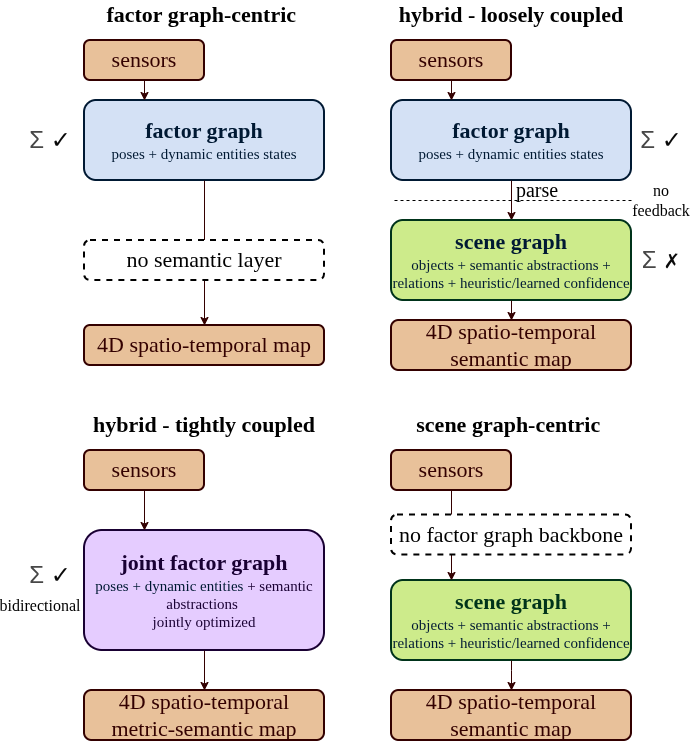
\includegraphics[width=0.9\columnwidth]{Figures/figure_architectural_patterns.png}
    \caption{Four distinct architectures have emerged throughout the literature for representing dynamic environment, specifically \textit{factor graph-centric} (top left), \textit{scene graph-centric} (bottom right), \textit{loosely coupled hybrid FG-SG} (top right) and \textit{tightly-coupled hybrid FG-SG} (bottom left).}
    \label{fig:architectural_patterns}
\end{figure}

\paragraph{Tightly-Coupled SLAMMOT (FG-centric)}
Systems in this pattern, like DynaSLAM II \cite{bescos_dynaslam_2021}, DynoSAM \cite{morris_dynosam_2025}, AirDOS \cite{qiu2022airdos}, BodySLAM \cite{henning_bodyslam_2022}, BodySLAM++ \cite{henning_bodyslam_2023}, Gou et al. \cite{gou_visual_2024}, adopt the joint-optimization approach detailed in Section \ref{sec:dynamics_representations_agents}, treating dynamic entities as first-class factor graph variables rather than outliers.% a probabilistic rigorous approach to dynamic agent handling.
%They jointly optimize camera pose, static landmarks, and dynamic entity trajectories within a unified factor graph, using spatio-temporal reprojection factors to introduce cross-terms that make self-localization and object tracking mutually reinforcing. 
%A defining characteristic of this pattern is that dynamic entities are treated as first-class factor graph variables rather than as outliers. 
The trade-off is that this template primarily addresses continuously moving agents, while semi-static displacement and long-term structural changes are typically outside its scope, and no explicit semantic abstraction layer is provided for higher-level reasoning tasks.

\paragraph{Layered Stack with FG Backbone ( loosely coupled hybrid FG-SG)}
Kimera \cite{rosinol_kimera_2021} and Hydra \cite{hughes_hydra_2022} exemplify a layered architecture in which a factor graph optimizer provides a globally consistent geometric foundation, while a separate scene graph parser constructs the semantic-relational superstructure. 
The advantage is modularity: the scene graph logic can be developed independently of the SLAM back-end. 
The disadvantage is one-directional information flow: the scene graph is informed by the factor graph, but semantic information rarely propagates back to improve localization, so geometric uncertainty never reaches the semantic layer.


\paragraph{Unified Optimizable Graph ( tightly-coupled hybrid FG-SG)}
S-Graphs \cite{bavle_s-graphs_2025} and DynEMo-SLAM \cite{giberna_dynemo-slam_2025} incorporate semantic entities directly as variables and factors within the same factor graph that optimizes robot poses. 
This enables bidirectional information flow: semantic structural priors constrain ego-trajectory estimation, while geometric observations refine semantic entity states. 
DynEMo-SLAM extends this template to dynamic entities by constraining entity pose variables with semantic motion priors and structural relations. 
The pattern is particularly expressive in environments where structural semantics are stable and informative, while its applicability to large-scale, dynamic outdoor settings, where the number and identity of semantic entities grow rapidly, has not yet been demonstrated.
%represent a tighter integration in which semantic entities are incorporated directly as variables and factors within the same factor graph that optimizes robot poses.
% This enables bidirectional information flow: semantic structural priors constrain ego-trajectory estimation, while geometric observation refine semantic entity states.
% Specifically, DynEMo-SLAM extends this template to dynamic entities by constraining entity pose variables with semantic motion priors and structural relations.
% The pattern is particularly expressive in environments where structural semantics are stable and informative. 
% However, its applicability to large-scale, dynamic outdoor settings, where the number and identity of semantic entities grow rapidly, has not yet been demonstrated. 

\paragraph{Belief-Augmented and Dynamic Scene Graph (SG-centric)}
DovSG \cite{yan_dynamic_2025}, Lost \& Found \cite{behrens_lost_2025}, BSG \cite{saucedo_estimating_2025}, Aion \cite{catalano_aion_2025}, and Functional Scene Graphs \cite{zhang_open-vocabulary_2025} emphasize the scene graph as a persistent and explicitly dynamic world model, maintained primarily through semantic reasoning and graph-level updates rather than joint probabilistic optimization.
Persistence, forgetting, and state transition are central to this pattern: Lost \& Found distinguishes object removal from occlusion through the containment mechanism described in Section \ref{sec:dyn_world_model_representations_scene_graphs}.
Aion further extends this paradigm by encoding temporal activity patterns directly into the scene graph structure. 
These approaches  support long-term object permanence, natural language grounding, and interaction aware updates. 
Their reliance on heuristic or learned confidence measures, rather than trajectory level covariances, reflects a different trade-off between semantic expressiveness and probabilistic state estimation.

% Several descriptive patterns emerge from the taxonomy. 
% \textbf{Factor-graph-based systems} predominantly focus on geometric consistency and probabilistic state estimation, often providing explicit uncertainty representations and strong guarantees for incremental inference. 
% These approaches naturally support continuous dynamics and tightly-coupled estimation of robot and object motion, but typically require additional abstraction layers to support high-level semantic reasoning.

% In contrast, \textbf{scene-graph-centric systems} emphasize structured, hierarchical representations of the environment, enabling symbolic queries, task-level reasoning, and interaction modeling. 
% These systems frequently support semi-static changes and long-term memory through explicit graph maintenance mechanisms, although uncertainty is often represented implicitly or heuristically rather than through fully probabilistic inference.

% \textbf{Hybrid architectures} combine these complementary strengths by grounding semantic entities in a probabilistic geometric backbone. 
% Such systems commonly employ factor graphs for metric consistency and temporal estimation, while leveraging scene graphs to organize entities across abstraction levels and support downstream decision-making. 
% The taxonomy shows that hybrid approaches tend to integrate incremental smoothing back ends with hierarchical graph structures and explicit maintenance policies, reflecting the increased complexity of jointly modeling geometry, semantics, and dynamics.

% Across all graph stacks, the comparison highlights consistent relationships between the type of dynamics addressed, the chosen association and inference strategies, and the intended downstream applications. 
% These recurring patterns provide a consolidated view of how graphical models are currently employed for dynamic world modeling in robotics.

% \subsection{Trends in Graph-based World Modeling}\label{sec:taxonomy_trends}


% \paragraph{From Closed-Vocabulary to Open-Vocabulary Association} 
% \textcolor{red}{\sout{Early dynamic SLAM systems defined a fixed ontology of entities types at design type, like pedestrians, vehicles, or furniture, and relied on classifiers trained on these predefined categories.
% More recent systems increasingly leverage vision-language embeddings, including CLIP-based representations and vision-language models, to support open-vocabulary perception and association. 
% Frameworks such as DovSG \cite{yan_dynamic_2025} and ConceptGraphs \cite{gu_conceptgraphs_2023} demonstrate that open-set object discovery and association can be integrated into real-time robotic systems, enabling world models to accommodate previously unseen categories without retraining.}}

% \paragraph{From Reactive Maps to Predictive Spatial Memory}
% \textcolor{red}{\sout{
% Early dynamic world models were predominantly reactive, updating internal representations only in response to incoming observations and answering queries about the current state of the environment.
% A clear trend in more recent work is the incorporation of predictive components that encode expectations about unobserved entities and future activity, of which Aion's flow statistics (discussed below) are a representative case\cite{catalano_aion_2025}.
% Belief Scene Graphs' blind nodes (Section \ref{sec:dyn_world_model_representations_scene_graphs}) similarly estimate likely object locations from learned co-occurrence patterns \cite{saucedo_estimating_2025}, while Gorlo et al. \cite{gorlo_long-term_2024} leverage relational scene context to forecast long-term human trajectories.
% Altogether, these approaches extend world models from reactive state estimates toward representations that encode spatio-temporal patterns. 
% }}

% \paragraph{From Static Hierarchy to 4D Spatio-Temporal Representations}
% \textcolor{red}{\sout{Conventional 3D scene graph formulations organize the environment into a spatial hierarchies, such as objects, places, rooms, and buildings, that are largely static in their structural definition.
% Recent work has shifted from this assumption by explicitly incorporating temporal information into the representation\cite{schmid_khronos_2024}.
% Aion\cite{catalano_aion_2025} is the clearest instance of this shift: by attaching time-dependent flow statistics directly to navigational nodes, it extends the scene graph into a four-dimensional representation that captures not only spatial structure but temporal patterns of activity.
% %, for instance, attaches time-dependent flow statistics directly to navigational nodes, effectively extending the scene graph into a four-dimensional representation that captures not only the spatial structure but also temporal patterns of activity.
% This shift reflects a broader trend toward world models that encode when and how frequently interactions occur, rather than treating temporal variation as a sequence of independent snapshots.}}


%%% OLD NOTES
% Hierarchical Abstraction: The shift from "flat" representations to hierarchical 3D Scene Graphs (3DSGs) allows robots to reason over spaces in terms humans understand (e.g., rooms, buildings) rather than just dense point clouds \cite{rosinol_3d_2020, rosinol_kimera_2021}.

% Uncertainty Modeling: While early systems like Kimera use explicit Bayesian updates for semantic mesh labeling \cite{rosinol_kimera_2021}, newer frameworks like Lost \& Found \cite{behrens_lost_2025} highlight that modeling uncertainty for tracked objects is a critical next step for handling ambiguous interactions.

% Efficiency in Inference: Morris et al. \cite{morris_importance_2024} demonstrate that using a Hybrid formulation (combining world-centric and object-centric views) significantly increases factor graph sparsity, allowing for incremental solvers like iSAM2 to achieve real-time performance that previously required heavy batch optimization.

% Open-Vocabulary Capabilities: Systems like DovSG \cite{yan_dynamic_2025} and ConceptGraphs \cite{gu_conceptgraphs_2023} leverage Vision-Language Models (VLMs) to handle object categories unforeseen at design time, making them far more adaptable to real-world household environments compared to older "closed-vocabulary" SLAM systems

% Geometric-Semantic Hybridization: The most robust systems, such as Kimera \cite{rosinol_kimera_2021} and DynoSAM\cite{morris_dynosam_2025}, leverage factor graphs as a low-level "geometric backbone" while employing 3D Scene Graphs (3DSGs) for high-level semantic reasoning. This allows for joint optimization of robot trajectories and dynamic agent motions, resolving the motion ambiguity inherent in dynamic SLAM.

% Persistence and Forgetting Policies: Lifelong autonomy frameworks like Lost \& Found \cite{behrens_lost_2025} implement specific logic to handle semi-static change. Decisions to maintain object permanence (via "contains" edges) or prune "stale" nodes are driven by geometric verification—distinguishing between "absence of evidence" (occlusion) and "evidence of absence" (removal) \cite{schmid_khronos_2024}.

% Probabilistic Expectation: Emerging works in Belief Scene Graphs utilize GCN-based link prediction to populate unobserved areas with "blind nodes"\cite{saucedo_estimating_2025}. This shifts the world model from a purely reactive map to a predictive memory structure capable of guiding active object search under partial observability.

% Transition to 4D Representations: Recent frameworks like Aion \cite{catalano_aion_2025} extend the hierarchical stack by attaching temporal flow dynamics (Maps of Dynamics) directly to navigational nodes. By learning directional flow statistics over daily or seasonal cycles, these 4D scene graphs enable proactive planning in highly populated, rhythmic environments.

% The "Moving" vs. "Movable" Distinction: Brink (2016)\cite{brink_using_2016} and Gomez et al. (2020)\cite{gomez_object-based_2020} move beyond simple outlier rejection by modeling an object's capability for movement (semi-static). This allows the robot to retain a chair in its map even when it is stationary, while remaining alert that its position might change.

% Complexity Management: Walcott-Bryant et al. (2012)\cite{walcott-bryant_dynamic_2012} highlight that for lifelong autonomy, a graph cannot grow indefinitely. They implement an explicit "forgetting" policy that prunes nodes where significant change has been detected, ensuring the optimization remains tractable.

% Decoupling Spatio-Temporal Inconsistencies: Khronos \cite{schmid_khronos_2024} introduces the concept of "object fragments" to factorize the spatio-temporal SLAM problem. By breaking observations into locally consistent fragments, the system can disentangle sensor noise from actual environmental changes.

% 4D Representations: Aion \cite{catalano_aion_2025} represents a significant shift by attaching temporal flow dynamics directly to the navigational nodes of a 3D scene graph. Instead of just tracking a single person, it learns the "rhythm" of the environment (e.g., a hallway that is busy every day at 9 AM), transforming a static 3DSG into a predictive 4D model.

% \begin{table*}[t]
%   \caption{TODOHow methods encode time, change, and maintenance in probabilistic (factor-graph) and structured (scene-graph) world models.}
%   \label{tab:taxonomy_dynamics}
%   \centering
%   \scriptsize
%   \setlength{\tabcolsep}{3pt}

%   \begin{tabularx}{\textwidth}{@{}l l l l l l l >{\raggedright\arraybackslash}X@{}}
%     \toprule
%     \textbf{Work} & \textbf{Temporal model} & \textbf{Change model} & \textbf{Existence} &
%     \textbf{Mode/state} & \textbf{Graph updates} & \textbf{Consistency} &
%     \textbf{Notes (what’s novel)} \\
%     \midrule

%     Behrens et al. (2025) &
%     \makecell[l]{Delayed online\\sliding window} &
%     \makecell[l]{Rigid 6DoF\\tracking} &
%     \makecell[l]{Heuristic\\interval} &
%     \makecell[l]{Open/closed\\(drawer)} &
%     \makecell[l]{Online relation\\updates} &
%     \makecell[l]{Transformable\\scene graph} &
%     \makecell[l]{Maintains object permanence for\\objects stored in drawers.} \\
%     \midrule

%     Bescos et al. (2020) &
%     \makecell[l]{Fixed temporal\\window (2s)} &
%     \makecell[l]{Constant-vel\\(motion)} &
%     \makecell[l]{Heuristic\\(keypoints)} &
%     \makecell[l]{3D bounding\\boxes} &
%     \makecell[l]{Dynamic keyframe\\insertion} &
%     \makecell[l]{Tightly-coupled\\joint BA} &
%     \makecell[l]{Mutual benefit between camera\\tracking and object tracking.} \\
%     \midrule

%     Brink (2016) &
%     \makecell[l]{Incremental BP\\(incremental)} &
%     \makecell[l]{Constant-vel\\+ accel} &
%     \makecell[l]{Binary latent\\variable ($x$)} &
%     \makecell[l]{Capable of\\move ($m$)} &
%     \makecell[l]{Incremental\\``forgetting''} &
%     \makecell[l]{Joint PGM\\segmentation} &
%     \makecell[l]{Explicitly models semi-static objects\\switching between states.} \\
%     \midrule

%     Morris et al. (2025) &
%     \makecell[l]{Incremental\\iSAM2} &
%     \makecell[l]{World-centric\\rigid motion} &
%     \makecell[l]{Heuristic\\tracklets} &
%     \makecell[l]{SE(3) pose\\+ motion} &
%     \makecell[l]{iSAM2 clique\\restructuring} &
%     \makecell[l]{Hybrid factor\\graph} &
%     \makecell[l]{Hybrid formulation improves sparsity\\for online incremental solving.} \\
%     \midrule

%     Rosinol et al. (2021) &
%     \makecell[l]{Fixed-lag (VIO)\\+ batch (DSG)} &
%     \makecell[l]{Continuous\\agent motion} &
%     \makecell[l]{Heuristic\\(semantic)} &
%     \makecell[l]{Panoptic\\labels} &
%     \makecell[l]{Mesh\\deformation} &
%     \makecell[l]{Hierarchical\\PGO} &
%     \makecell[l]{Integrates visual-inertial SLAM with\\dense human mesh (SMPL) tracking.} \\
%     \midrule

%     Gomez et al. (2020) &
%     \makecell[l]{Multi-session\\(offline sessions)} &
%     \makecell[l]{Relocated\\furniture} &
%     \makecell[l]{Probabilistic\\presence} &
%     \makecell[l]{Active vs.\\inactive} &
%     \makecell[l]{Online object\\merging} &
%     \makecell[l]{Object-based\\pose graph} &
%     \makecell[l]{Infers object ``movability'' based on\\long-term session experience.} \\
%     \midrule

%     Catalano et al. (2025) &
%     \makecell[l]{FreMEn frequency\\model} &
%     \makecell[l]{Navigational\\motion flows} &
%     \makecell[l]{Position-invariant\\hashing} &
%     \makecell[l]{Activity\\histograms} &
%     \makecell[l]{Temporal ownership\\transfer} &
%     \makecell[l]{Hydra-integrated\\PGO} &
%     \makecell[l]{First unification of Maps of Dynamics\\(MoD) and 3D Scene Graphs.} \\
%     \midrule

%     Walcott-Bryant et al. (2012) &
%     \makecell[l]{Incremental\\smoothing} &
%     \makecell[l]{Low-dynamic\\structural} &
%     \makecell[l]{Change node\\indicator ($c$)} &
%     \makecell[l]{Static, Added,\\Removed} &
%     \makecell[l]{Stale node\\pruning} &
%     \makecell[l]{Pose-graph\\optimization} &
%     \makecell[l]{Reduces graph size by removing stale\\nodes that no longer match reality.} \\
%     \bottomrule
%   \end{tabularx}

%   \vspace{2pt}

%   \begin{tabularx}{\textwidth}{@{}l >{\raggedright\arraybackslash}X@{}}
%     \textbf{Entries:} &
%     \textbf{Temporal model} (filtering vs smoothing, incremental vs batch);
%     \textbf{Change model} (continuous motion, displacement, structural change);
%     \textbf{Existence} (explicit latent variable or heuristic);
%     \textbf{Mode/state} (discrete states like open/closed);
%     \textbf{Graph updates} (node/edge addition/removal, compression);
%     \textbf{Consistency} (pose-graph optimization only vs joint graph optimization).
%     \\
%   \end{tabularx}
% \end{table*}

